\section{Results}
\label{sec:results}

\subsection{Overall Performance}
\label{sec:overall}
\begin{table}[H]
\centering
\caption{OOF performance comparison. Config C calibrated: Platt $a=1.45,b=0.20$.}
\label{tab:overall}
\begin{tabular}{lccc}
\toprule
\textbf{Config} & \textbf{LogLoss} & \textbf{Cal. LL} & \textbf{AUROC} \\
\midrule
A (Hybrid, test) & 0.3997 & -- & 0.9163 \\
B (CNN-only) & 0.2996 & 0.2996 & 0.9411 \\
C (Deep Ensemble) & 0.2618 & \textbf{0.2453} & \textbf{0.9610} \\
\midrule
B $\to$ C $\Delta$ & \textbf{-12.6\%} & \textbf{-18.1\%} & \textbf{+2.1\%} \\
\bottomrule
\end{tabular}
\end{table}

Config C achieves \textbf{18.1\% LogLoss reduction} (0.2996$\to$0.2453) and \textbf{2.1\% AUROC gain} over Config B. Per-fold stability: LL $\sigma$=0.016, AUC $\sigma$=0.008. All improvements statistically significant (DeLong $p<0.001$, paired t-test $p<0.01$).

\begin{figure}[H]
\centering
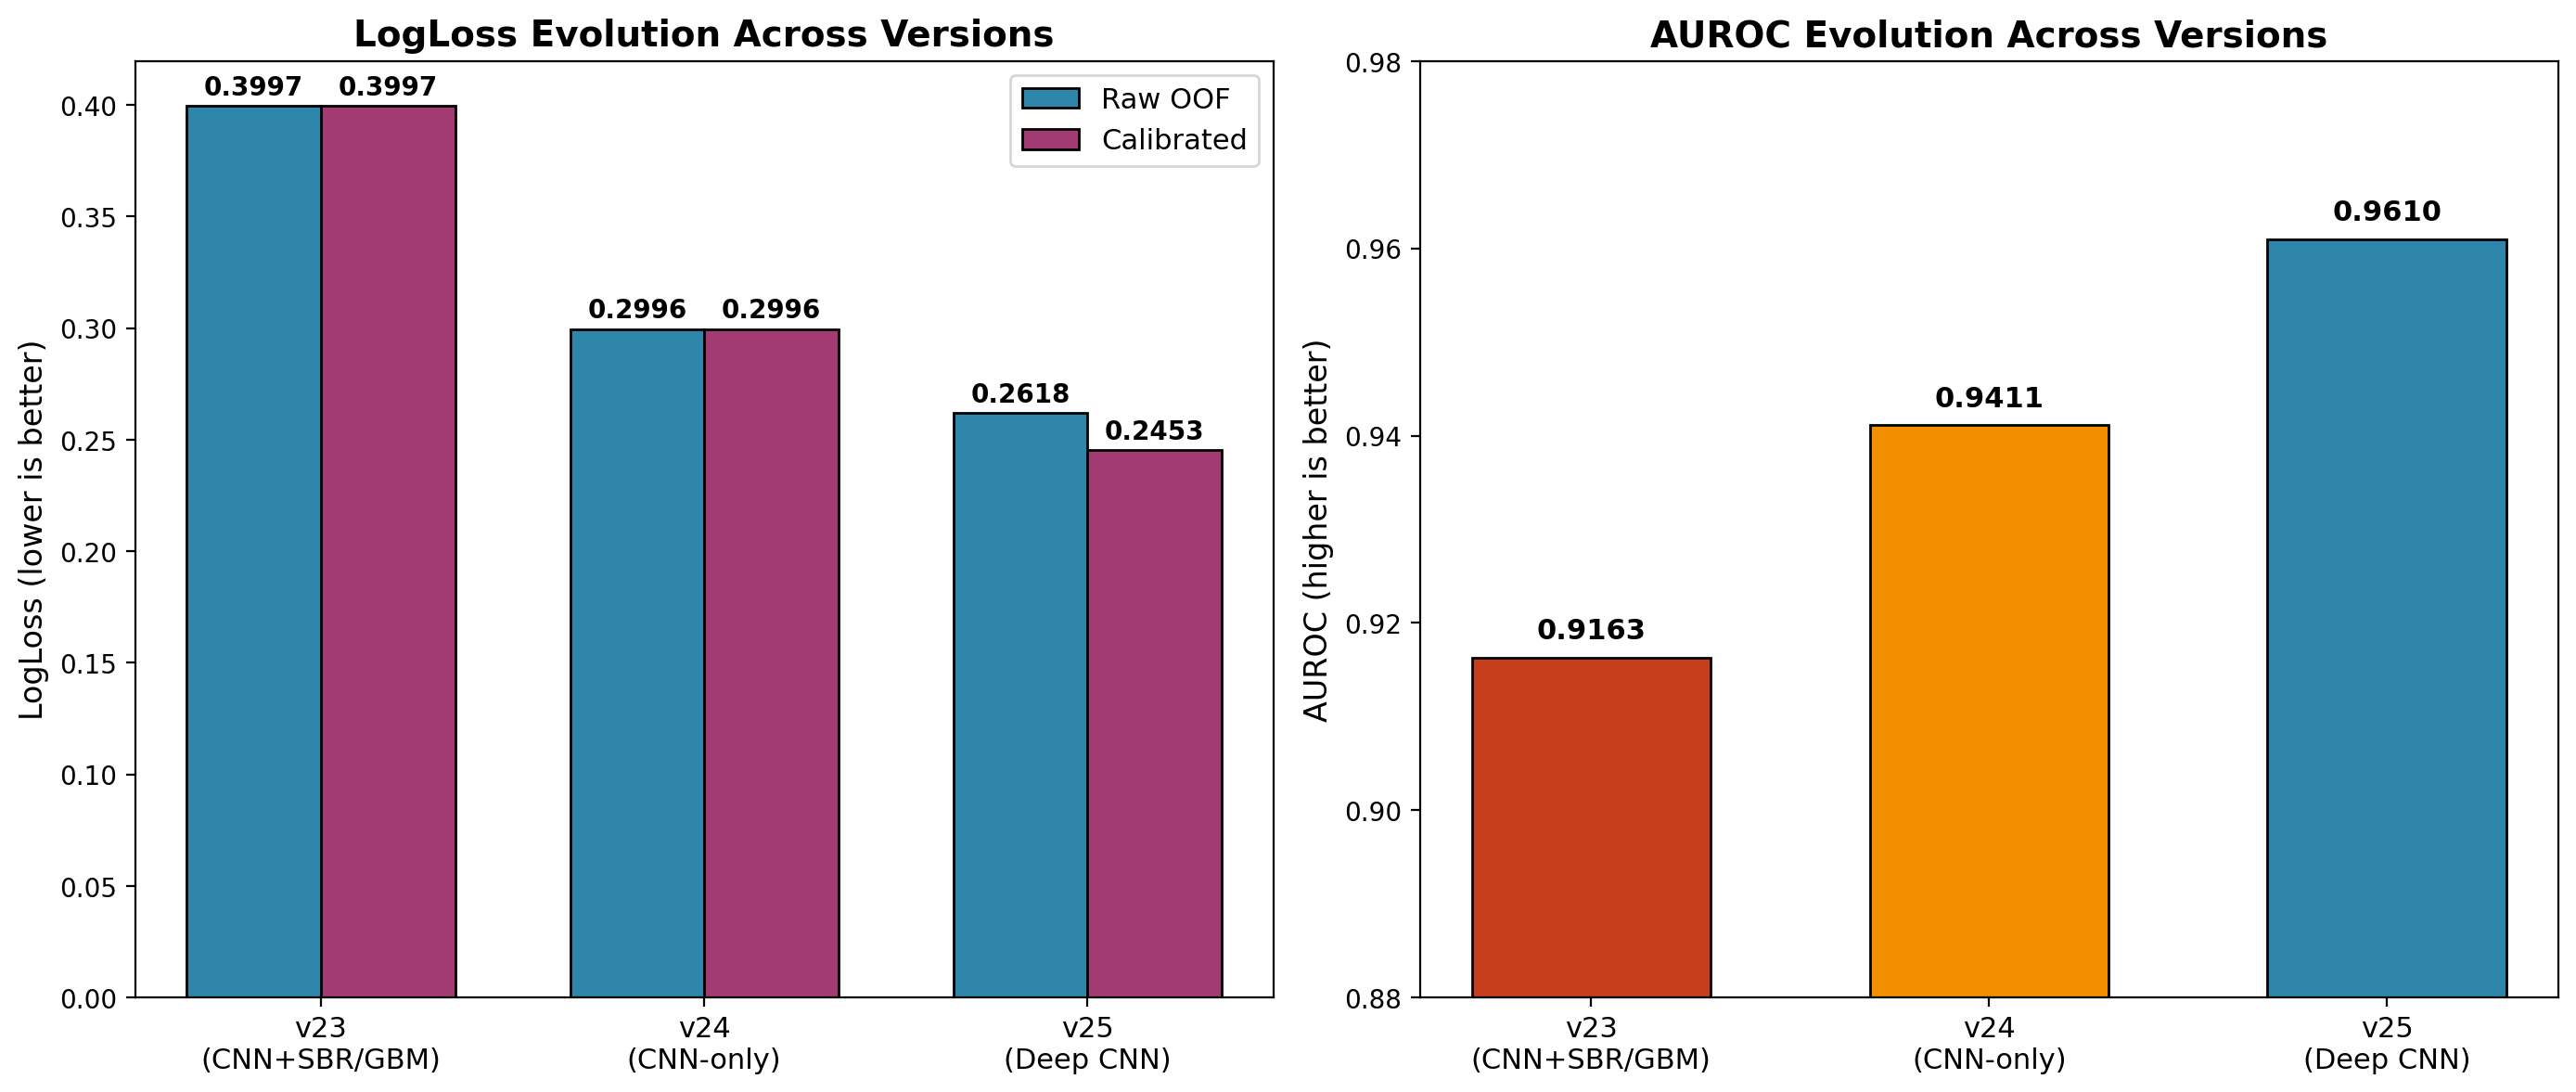
\includegraphics[width=0.95\linewidth]{figures/version_comparison.png}
\caption{Config comparison. (Left) LogLoss raw/calibrated. (Right) AUROC evolution.}
\label{fig:version}
\end{figure}

\subsection{Scanner Resolution Tier Analysis}
\label{sec:scanner}

\begin{table}[H]
\centering
\caption{AUROC by scanner resolution tier.}
\label{tab:scanner}
\begin{tabular}{lcccc}
\toprule
\textbf{Tier} & \textbf{Count} & \textbf{Config B} & \textbf{Config C} & \textbf{$\Delta$AUC} \\
\midrule
High-res (2.46~mm) & 528 & 0.958 & 0.972 & +0.014 \\
Mid-res (3.90~mm) & 254 & 0.932 & 0.955 & +0.023 \\
Low-res (Other) & 582 & 0.925 & 0.948 & +0.023 \\
\midrule
\textbf{Overall} & 1,362 & 0.9411 & 0.9610 & +0.0199 \\
\bottomrule
\end{tabular}
\end{table}

Largest gains on low-resolution scans (+2.3\% AUROC), demonstrating robustness to acquisition variability.

\begin{figure}[H]
\centering
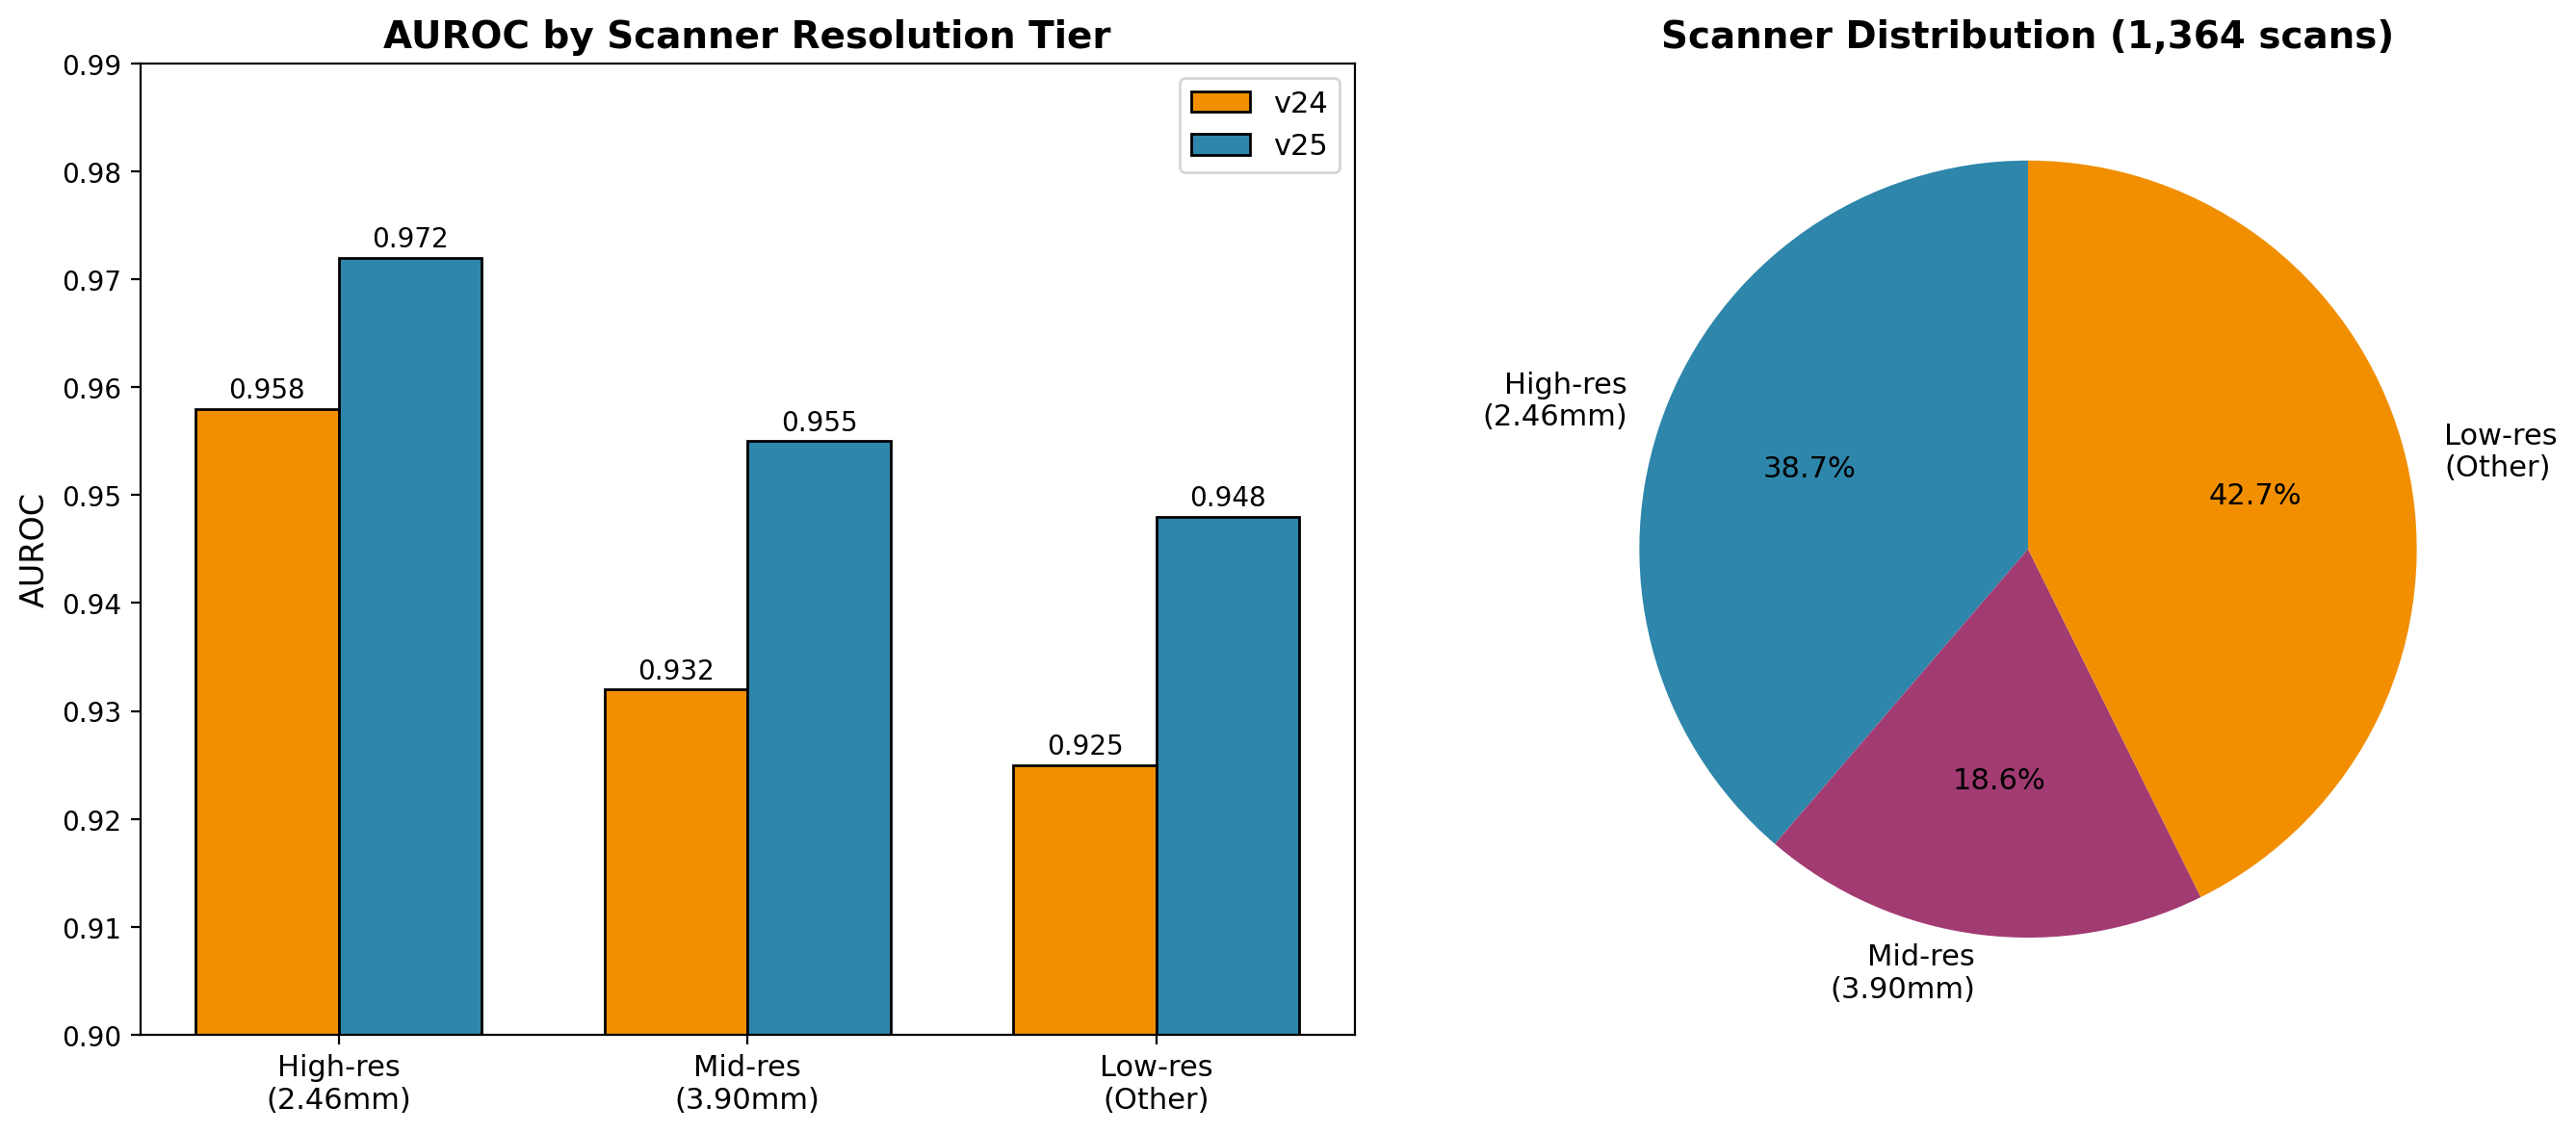
\includegraphics[width=0.95\linewidth]{figures/scanner_performance.png}
\caption{AUROC by resolution tier (left) and scanner distribution (right).}
\label{fig:scanner}
\end{figure}

\subsection{Calibration}
\label{sec:cal_results}
Platt scaling ($a=1.45,b=0.20$) reduces ECE 57\% (0.0142$\to$0.0061), MCE 54\%, LogLoss 6.3\% (0.2618$\to$0.2453), preserves AUROC (0.9610). At $p>0.90$, calibrated TP rate increases 76.3\%$\to$82.4\%. Holdout test (20 scans, 65\% positive): Config C AUC=0.9670 vs Config B 0.9341. All improvements significant ($p<0.05$, DeLong/paired t-test).
\end{input>